% MODELO CONEM 2016
\documentclass[10pt,fleqn,a4paper]{article}
\usepackage{abcm}
\usepackage{float}

\begin{document}
    
    % CABEÇALHO
    \fancypagestyle{firststyle}
	{
   		\lhead{\emph{Anais do XXIV Encontro de Iniciação Científica e Pós-Graduação do ITA - XXIV ENCITA / 2018
	Instituto Tecnológico de Aeronáutica, São José dos Campos, SP, Brasil, XXIV 18 de outubro de 2018}}  
	}
    \thispagestyle{firststyle}
    \vspace{-.5cm}
    \hspace{-.8cm}
    \begin{tabular}{p{\textwidth}}
    \begin{center}
    \vspace{-.6cm}
    \title{Estratégia de time de Robôs Very Small Size}
    \end{center}
    \textbf{Igor Mourão Ribeiro}\\
    \small{Instituto Tecnológico de Aeronáutica}\\
    \small{Rua H8C, 317, CTA}\\
    \small{12.228-462 - São José dos Campos/SP}\\
    \small{Bolsista PIBIC - CNPq}\\
    \small{igormr98mr@gmail.com}\\
    \\ 
    \textbf{Paulo Marcelo Tasinaffo}\\
    \small{Instituto Tecnológico de Aeronáutica}\\
    \small{Divisão de Ciência da Computação}\\
    \small{Praça Marechal Eduardo Gomes, 50}\\
    \small{12.229-900 – São José dos Campos / SP}\\
    \small{tasinaffo@ita.br}\\
    \\ 
    \textbf{Marcos Ricardo Omena de Albuquerque Máximo}\\
    \small{Instituto Tecnológico de Aeronáutica}\\
    \small{Divisão de Ciência da Computação}\\
    \small{Praça Marechal Eduardo Gomes, 50}\\
    \small{12.229-900 – São José dos Campos / SP}\\
    \small{maximo.marcos@gmail.com}\\
    \\
    \abstract{\textbf{Resumo:} O desenvolvimento de uma estratégia robusta e consistente para um time completo de robôs jogadores de futebol da categoria "Very Small Size" é fundamental para ganhar as partidas. Após uma fase de pesquisa, foi decidido usar o método da Behavior Tree (árvore de comportamentos) para realizar a tomada de decisões do time. Em seguida, foi escolhido três papeis para os jogadores: goleiro, principal e auxiliar. Depois, foi desenvolvido uma árvore de comportamentos para cada um deles, além de um técnico responsável por garantir troca dinâmica de papeis. O critério usado para avaliação do algoritmo foi o seu desempenho em partidas simuladas e em competições nacionais.}\\
    \keywords{\textbf{Palavras-chave:} robótica, estratégia, tomada de decisão}\\
    \end{tabular}

    \section{INTRODUÇÃO}
        	
	No contexto do futebol de robôs, a tomada de decisão traz muitos desafios. A estratégia consiste no fato de se implementar um algoritmo que consiga utilizar o planejamento de trajetórias do robô da melhor maneira possível. Isso nos traz a um desafio de nível de abstração mais alto: decidir qual a melhor decisão que cada robô pode tomar em um certo momento considerando limitações de trajetórias possíveis de serem seguidas.

	Nesse projeto, trabalhou-se com os robôs da competição IEEE Very Small Size (VSS): uma competição de futebol de robôs completamente automatizada em que cada robô tem como tamanho máximo um cubo de 7,5 cm de aresta. O campo de futebol possui 1,5 m de comprimento e 1,3 m de largura. Cada time tem 3 jogadores: que podem assumir posições dinâmicas, como goleiro e atacante, ao decorrer de uma partida. Uma câmera proporciona a visão aérea com as posições de todos os elementos da partida. As regras completas podem ser lidas em \cite{CBR2008}.

\begin{figure}[H]
	\centering
	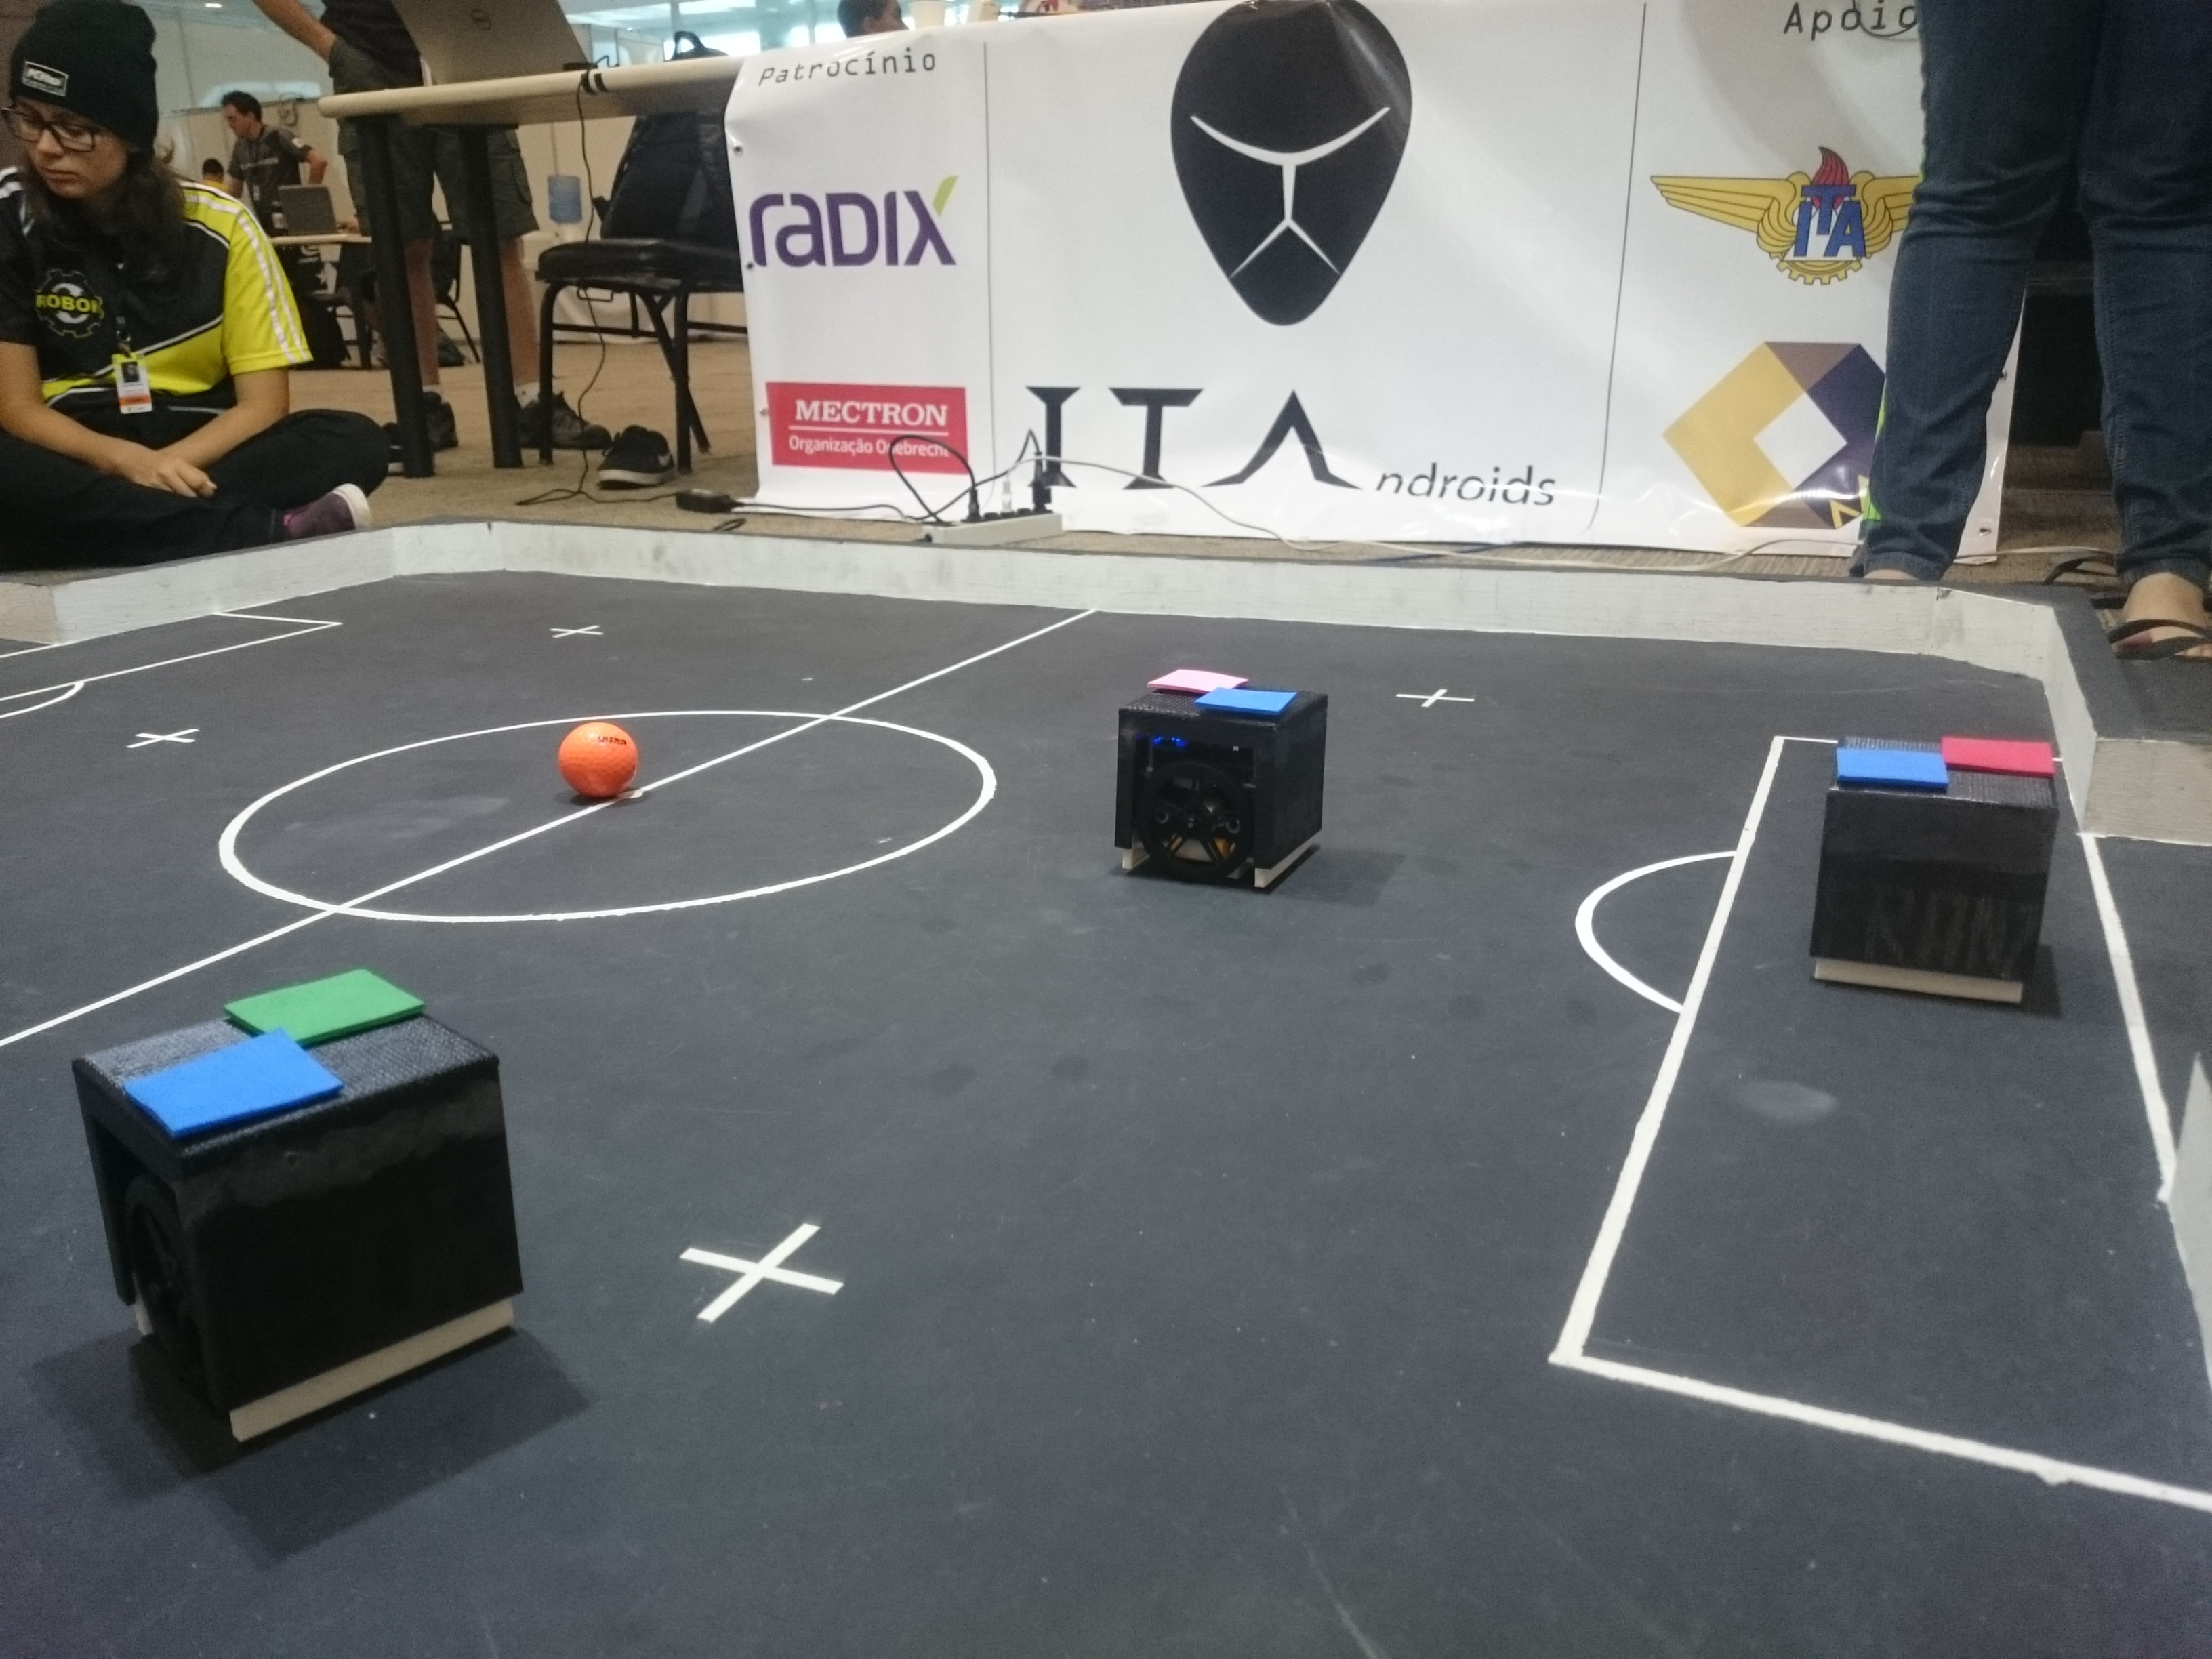
\includegraphics[width=0.5\textwidth]{figures/vss-min.JPG}
   \caption{Robôs da ITAndroids da categoria IEEE VSSS.} \label{fig:vss}
\end{figure}

	A Figura \ref{fig:vss} mostra os robôs usados nas competições. A visão computacional utilizada pela equipe ITAndroids pode ser encontrada com mais detalhes em \cite{zickler2009ssl} e utiliza uma câmera no topo do campo que repassa informações para um computador processar, como visto na Figura \ref{fig:funcioamento}.

\begin{figure}[H]
	\centering
		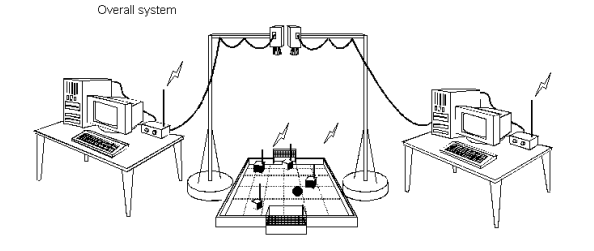
\includegraphics[width=0.7\textwidth]{figures/overview.png}
  \caption{Representação do funcionamento técnico de um jogo de VSS.}
	\label{fig:funcioamento}
\end{figure}

Cada robô foi projetado com duas rodas laterais e duas esferas livres à frente e atrás para manter o equilíbrio. Essa característica o torna um robô diferencial. Ou seja, temos o controle sobre as velocidades linear e angular, mas não é possível mover o robô para os lados. A linguagem utilizada para o projeto foi C++, pois é uma linguagem que tem uma velocidade de execução alta e tem boa escalabilidade para um projeto grande. 

Nesse contexto, surgem várias questões a serem resolvidas para se ter um time vencedor. Nesse projeto, será abordado o seguinte problema de estratégia: dada a posição e a velocidade de cada robô e da bola, deve-se escolher qual posição um determinado robô irá, com qual controlador  e qual planejamento de trajetórias utilizar. Deve-se também montar um plano para ações futuras, planejando uma sequência de posições que o robô deve ir para efetuar um gol.

O algoritmo de estratégia deve executar em tempo de execução de, no máximo, 10 ms para todo o time, que é o tempo de amostragem da câmera descontado do tempo de processamento da visão computacional. A maior parte desse tempo é gasto com o planejamento de trajetórias usado, que é o Rapidly-exploring Random Tree (RRT). O tempo para cada execução de um RRT é de 1 ms, de acordo com \cite{franzoni_rrt}, limitando a em torno de um limite de doze chamadas do algoritmo por execução completa da estratégia, com uma margem de erro de trinta e três porcento. Ressalta-se a importância de não ultrapassar esse tempo máximo, já que se isso acontecer perde-se uma imagem da câmera e o funcionamento do jogo é realizado de forma atrasado.

Deve-se, então, ser montado um esquema de posicionamento dinâmico em que não existam nem atacante, nem zagueiro, nem goleiro fixos, mas sim, que as posições dependam e se adaptem com a posição de jogo, garantindo que os três jogadores possam estar mais bem posicionados e tenham liberdade para escolherem suas próximas ações. Isso deve ser feito porque o esquema de posicionamento fixo não funciona muito bem no contexto da categoria Very Small Size, já que limita muito a capacidade ofensiva e defensiva do time.

Para resolver esse problema, foi escolhido como principal algoritmo para a tomada de decisão a Behavior Tree. Esse algoritmo foi escolhido dentre de opções como Máquina de Estados Finita e Árvore de Comportamentos. Uma introdução a esses assuntos pode ser encontrada em \cite{orozcomaquinas} para máquina de estados finita e em \cite{decision_tree} para Árvore de Comportamentos. A escolha é embasada na decisão de um time referência no futebol de robô mundial, o Near East University team: the NEUIslanders, como descrido em \cite{NEUIslanders_ssl}.

Esse trabalho traz como contribuição a implementação do método Behavior Tree para a categoria Very Small Size, sendo a primeira publicação científica desse tema na literatura.

\subsection{Behavior Tree}

Para se construir uma Behavior Tree (BT), é preciso primeiro entender o básico de sua estrutura. Uma BT é uma Árvore no sentido dado pela teoria dos grafos, como explicado em \cite{west2001introduction}. Por definição, cada nó dessa árvore será chamado de behavior (comportamento).

Os nós de uma Behavior Tree são diferenciados em dois tipos: os nós folhas, que são os nós da árvore que não tem filhos e os nós compostos, que podem ter um ou mais filhos.

Todos os nós retornam, no final de sua execução, um dos três estados a seguir: TRUE, FALSE ou RUNNING, para indicar, respectivamente, que o nó foi terminado com sucesso, que foi terminado sem sucesso ou que o algoritmo deve executar esse nó por pelo menos mais uma iteração.

\subsubsection{Nós Folha}

Os nós folha são os nós terminais da Árvore e eles que representam as ações mais baixo níveis e concretas da estratégia. São divididas em dois tipos: nós de ação e nós condicionais.

\textbf{Nós de Ação} São os nós que de fato realizam uma ação, como se movimentar até a bola.

\textbf{Nós condicional} São nós que apenas retornam um estado sem realizar nenhuma ação concreta, como checar se o time está atacando. São usados para controlar quais nós serão executados em conjunto com os nós compostos.

\subsubsection{Nó composto}

Nós compostos são os nós intermediários da árvore, que  são responsáveis por escolher quais os nós que serão executados. São completamente reutilizáveis no sentido que apenas uma implementação de cada tipo de nó composto deve existir e ela poderá ser usada em diversas partes do código. Os principais tipos desses nós que foram usados para a estratégia estão listados a seguir:

\textbf{Selector Behavior} Nesse behavior, é selecionado um de seus filhos para ser acessado a seguir. Ele é usado quando tem-se várias maneiras de se realizar uma mesma ação e deve-se escolher a melhor delas em uma determinada situação. Ele funciona executando os filhos em uma determinada ordem e, assim que um dos filhos retorna TRUE ou RUNNING, esse nó retorna o mesmo valor. Se um filho retornar FALSE, o próximo filho será executado. Caso nenhum filho seja sucedido ou retorne que deve ser executado mais um vez, o nó retorna FALSE.

\textbf{Sequence Behavior} Esse nó executa cada um dos seus filhos em uma sequência bem definida e fixa. Ele é usado para fazer ações sequenciadas para completar um objetivo maior, por exemplo: chutar a bola para o gol oponente requer que o robô aliado esteja atrás da bola, o que significa que chegar atrás da bola e, em seguida, chutar a bola representam ações sequenciadas. Ele funciona de forma que, quando um filho retorna RUNNING ou FALSE, o behavior retorna o mesmo valor e, quando um filho retorna TRUE, ele avança para o próximo filho. Se todos os filhos retornarem TRUE, o behavior é bem sucedido e também retorna TRUE.

\textbf{Parallel Behavior} O objetivo desse nó é executar todos os seus filhos ao mesmo tempo, fato que pode ser obtido ao utilizar-se de processamento paralelo ou não. Na implementação desse trabalho foi usado a versão não paralela do algoritmo. Se um filho retorna FALSE, o behavior retorna FALSE. Se todos os filhos retornarem TRUE, o behavior retorna TRUE. Em todas as outras situações, o behavior retorna RUNNING e continua sua execução por pelo menos outra iteração.

\textbf{Decorator} O nome para esse behavior é inspirado no conceito de Decorator em Software Design Pattern, que pode ser estudado em \cite{hunt2013gang}. No contexto da Behavior Tree, esse nó tem apenas um filho e ele modifica o comportamento do filho de alguma maneira. Um decorador pode ser diversos tipos, mas os mais usados no projeto foram:

\begin{enumerate}
\item AlwaysFail e AlwaysSucceed: que fazem que o filho sempre retorne FALSE ou sempre retorna TRUE respectivamente.
\item UntilFail e UntilSucceed: fazem que o fiho sempre retorne RUNNING a não ser que ele retorna FALSE ou TRUE, respectivamente.
\item Invert: muda o retorno do filho de FALSE para TRUE e TRUE para FALSE.
\end{enumerate}

\subsection{Técnico}

Uma Behavior Tree, que embora consegue modelar comportamentos complexos com facilidade, nem sempre é a melhor escolha para determinadas situações. Por isso, a estratégia foi dividida em níveis de abstrações diferentes, em que um Técnico, representado pela classe Coach, seria responsável por escolher e administrar quais árvore cada um dos três jogadores deveria usar no momento.
Com essa implementação, tem-se um agente externo controlando a função dos jogadores por meio da escolha de uma BT, que pode ser uma árvore para um goleiro, para um principal e para um auxiliar. Isso significa que, em um determinado momento, o técnico pode escolher que o time tenha 1 goleiro, 1 principal e 1 auxiliar a até mesmo 3 principais ao mesmo tempo. Os requisitos esperados para cada um desses papéis será abordado a seguir. Além disso, também é função do técnico escolher o papel de cada jogador a cada iteração do código, de modo que as posições dos jogadores não sejam fixas ao decorrer do jogo.

    \section{RESULTADOS OBTIDOS}
        
	Os resultados a seguir foram obtidos estudando o comportamentos de equipes adversárias na competição, além de diversos testes com o time de robôs da ITAndroids contra si mesmo em simulações computacionais em um simulador feito pela própria equipe, como mostrado na Figura \ref{fig:simulator}.

\begin{figure}[H]
	\centering
	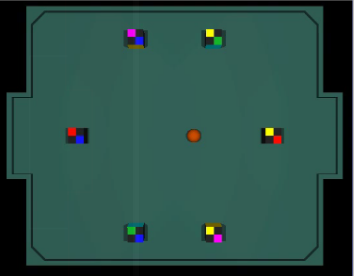
\includegraphics[width=0.6\textwidth]{figures/SimulatorWithoutButtons.png}
	\caption{Simulador da ITAndroids.}
	\label{fig:simulator}
\end{figure}

\subsection{Goleiro}

O goleiro é o jogador que deve ficar próximo ao gol aliado com o objetivo de proteger o gol de ataques oponentes. 
A BT criada para o goleiro está representada na Figura \ref{fig:goalier_bt}.

\begin{figure}[H]
	\centering
	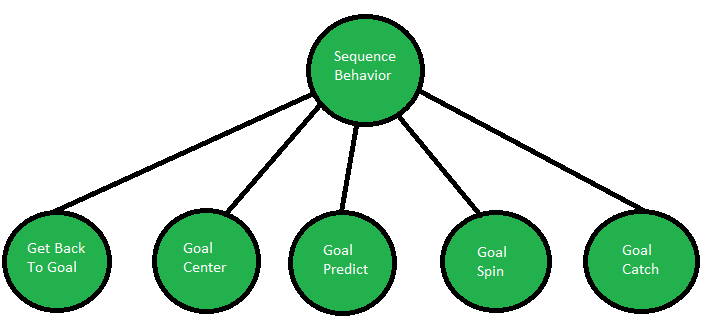
\includegraphics[width=0.8\textwidth]{figures/Goalier_BT.png}
   	\caption{Behavior Tree para o goleiro.} \label{fig:goalier_bt}
\end{figure}

Como visto, ela é composta por um nó do tipo Sequence Behavior, que irá executar os seus filhos em sequência. Esse papel, então, executa as seguintes ações prioritando as primeiras a aparecerem na seguinte lista:

\begin{itemize}

\item \textbf{Get Back to Goal Behavior} Volta para o gol, caso que, se por algum motivo ele esteja fora do próprio.

\item \textbf{Goal Center} Fica centralizado no gol quando a bola estiver longe, de forma que o jogador possa rapidamente ir para qualquer um dos lados quando a bola se aproximar.

\item \textbf{Goal Predict} Prediz para onde a bola irá quando ela estiver rápida e longe do gol.

\item \textbf{Goal Spin} Gira quando está perto da bola e não tem oponente perto da bola para jogá-la para longe.

\item \textbf{Goal Catch} Comportamento que o goleiro deverá fazer quando não fizer nenhum outro, por isso sua última posição na sequência. Ele acompanha o movimento da bola com o goleiro sobre a linha do gol.

\end{itemize}



\subsection{Principal}

O jogador com o papel de Principal é o jogador mais ativo do time, que deve estar constantemente avançando em direção a bola. Esse papel e o goleiro são as únicas posições que efetivamente deverão tocar na bola. A árvore \ref{fig:principal_bt} foi desenvolvida para o principal, sendo a árvore mais complexa dentre os papéis.

\begin{figure}[H]
	\centering
	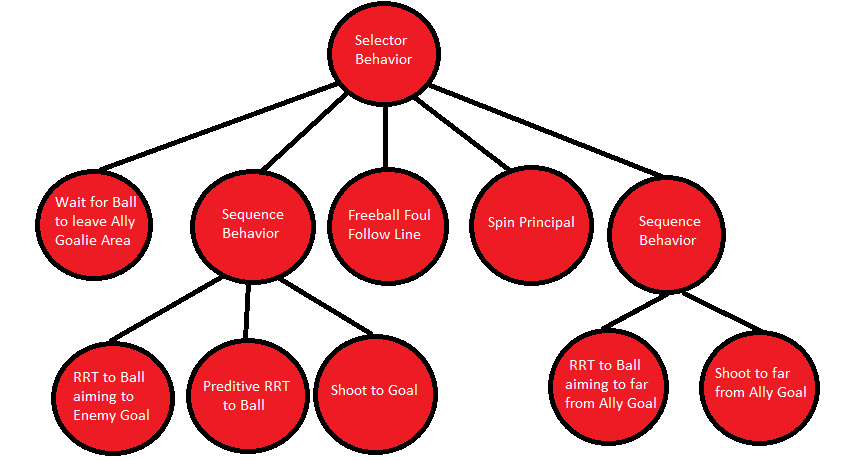
\includegraphics[width=0.8\textwidth]{figures/Principal_BT.png}
   	\caption{Behavior Tree para o principal.} \label{fig:principal_bt}
\end{figure}   

Conforme a Figura \ref{fig:principal_bt}, a raiz da árvore do principal é um Selector Behavior que escolhe uma das ações a ser realizada. Essa BT tem mais dois outros nós compostos, que são dois Sequence Behavior usados para o posicionamento atrás da bola, seguido pelo chute. Uma descrição dos nós folha utilizados se encontra abaixo:

\begin{itemize}

\item \textbf{Wait for Ball to leave Ally Goalie Area} Esse Behavior utiliza a Triangução de Delaunay. Esse comportamento deve evitar que o jogador entre na área do goleiro para não sofrer penâlti, conforme descrito na Figura \ref{fig:penalty}. O jogador se pocionará de acordo com posições escolhidas pelo usuário, calibradas com um arquivo de configuração .txt.

\begin{figure}[H]
	\centering
	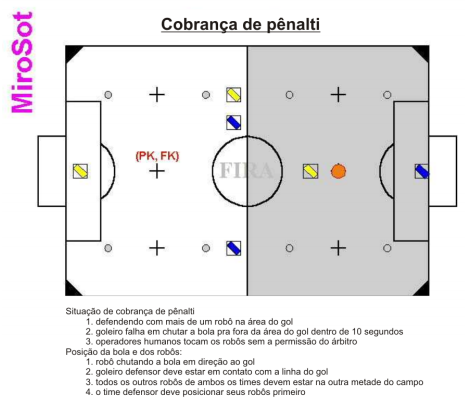
\includegraphics[width=0.7\textwidth]{figures/campo_penalty.png}
   \caption{Descrição da penalidade pênalti.} \label{fig:penalty}
\end{figure}

\item \textbf{RRT to Ball aiming to Enemy Goal} Irá usar o algoritmo de planejamento de trajetórias RRT para se deslocar atrás da bola com direção apontando para o gol oponente. Usado para se aproximar da bola e, em seguida, trocar para o próximo behavior, o Predictive RRT to Ball.

\item \textbf{Predictive RRT to Ball} Usa uma predição linear considerando que a bola continuará na mesma velocidade. Usado para se chegar na bola com mais precisão quando próximo a ela. Chega atrás da bola mirando para o gol.

\item \textbf{Shoot to Goal} Esse behavior só é chamado quando o jogador já está alinhado com a bola e o gol oponente. Esse comportamento acelera rapidamente o robô em linha reta para chegar no gol com uma velocidade alta.

\item \textbf{Free Ball Foul Follow Line} Esse behavior é um específico para situações de falta do tipo Bola Livre, conforme descrito na Figura \ref{fig:bola_livre}. Quando for detectado uma dessas posições, o jogador deve acelerar o mais rápido possível em direção à bola para ter o controle dela antes do oponente.

\begin{figure}[H]
	\centering
	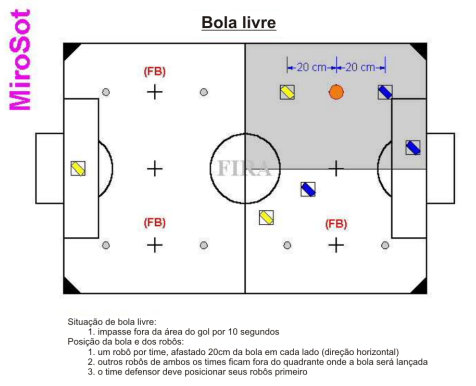
\includegraphics[width=0.7\textwidth]{figures/bola_livre.png}
   \caption{Descrição da penalidade bola livre.} \label{fig:bola_livre}
\end{figure}

\item \textbf{Spin Principal} Esse nó deve ser chamado quando a bola estiver em um dos quatros campos do campo. Caso seja um campo defensivo, o jogador irá girar para jogar a bola para frente; caso seja um na zona de ataque, o jogador girará para por a bola no centro do campo e continuar o ataque.

\item \textbf{RRT to Ball aiming to far from Ally Goal} Irá usar o algoritmo de planejamento de trajetórias RRT para se deslocar atrás da bola com direção apontando para a zona de ataque (longe do gol aliado). Usado para se aproximar da bola e se posicionar para, em seguida, chamar o Behavior Shoot to Far from Ally Goal.

\item \textbf{Shoot to Far from Ally Goal} Esse behavior só é chamado quando o jogador já está alinhado com a bola e o para frente (para longe do gol aliado). Esse comportamento acelera rapidamente o robô em linha reta para pôr a bola na zona de ataque.

\end{itemize}


\subsection{Auxiliar}

	O auxiliar é um papel que tem apenas uma função: posicionar-se da melhor forma possível para manter um ataque consistente. A ideia é que, caso a situação seja oportuna, o auxiliar se torne o principal e comece a atacar a bola. Para escolher a posição que o auxiliar deverá ficar em uma determinada situação de jogo, foi utilizado a Triangulação de \cite{delaunay34} sobre o grafo de \cite{voronoi08}. Esse algoritmo foi aplicado similarmente a \cite{akiyama2007multi}, relativo também à futebol de robôs.

	A Behavior Tree do auxiliar, por sua vez, é muito simples, representada por apenas um nó que tem como função se posicionar em lugar ótimo. Sua árvore, é representada simplesmente pela Figura \ref{fig:auxiliar_bt}.

\begin{figure}[H]
	\centering
	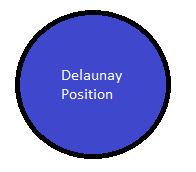
\includegraphics[width=0.3\textwidth]{figures/Auxiliar_BT.png}
   \caption{Behavior Tree para o auxiliar.} \label{fig:auxiliar_bt}
\end{figure}

	\section{CONCLUSÕES}
	Nesse artigo, apresentou-se uma implementação do método Behavior Tree para a categoria de futebol de robôs Very Small Size Soccer, que foi descrita, brevemente, o seu funcionamento. Foi mostrado o esquema de papéis utilizado bem como a Árvore de Comportamentos implementada para cada um deles, além de uma descrição detalhada sobre todos os nós das árvores.
	
	O projeto de Iniciação Científica apresentou bons resultados, especialmente quanto à vitória da equipe do ITA até às quartas de final da CBR 2017, rendendo o sétimo lugar à equipe dentre mais de 25 equipes participantes. Além do fato de que a ITAndroids conquistou o primeiro lugar na competição nacional de VSSS Copa Turing 2017, que ocorreu no final de setembro de 2017.

	Do ponto de vista técnico, o uso do algoritmo da Behavior Tree, já consagrado e usado por times de nível mundial, se mostrou factível e funcional em partidas reais de competições. Contudo, problemas como pouca escalabilidade e pouca reutilizabilidade se mostraram presentes na estratégia desenvolvida. Isso significa que mudanças ainda deverão ser feitas nas BT, principalmente a respeito do uso de mais nós do tipo paralelo para remover esses problemas citados.

    \section{AGRADECIMENTOS}
    
	Agradeço ao CNPq, pelo apoio financeiro e motivacional.
	
	Agradeço à ITAndroids, equipe que representa o ITA na competição da LARC/CBR, pela ideia do projeto, pela disponibilidade do robô real para implementação e oportunidade de aplicação dos métodos estudados.

	Agradeço ao professor doutor Paulo Marcelo Tasinaffo, meu orientador, e ao professor doutor Marcos Ricardo de Omena Máximo, co-orientador, ambos da Divisão da Ciência da Computação do ITA, pelo apoio nos estudos e no desenvolvimento do projeto.

    % REFERÊNCIAS
    \section{REFERÊNCIAS}
        \bibliographystyle{abcm}
        \bibliography{bibliografia}

    \section{RESPONSABILIDADE AUTORAIS}
    
        Os autores são os únicos responsáveis pelo conteúdo deste trabalho.

\end{document}